\section{Results}
\label{sec:result}
\subsection{RQ1. Change patterns}
\label{sec:result:pattern}


%The taxonomy includes change of lock type, change of lock variable, synchronization addition, synchronization removal, lock release, volatile addition, volatile removal, class replacement, thread-safe class replacement, thread management, thread status management,

%\begin{table*}
%\zhong{Please delete this table.}
%	\centering
%	\caption{Taxonomy}
%	\begin{tabular}{|c|c|c|}\hline
%		Type&Example&Occurrence\\\hline
%		Changing lock type&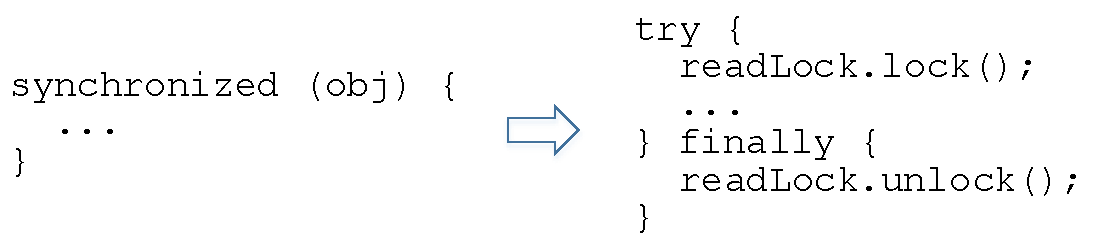
\includegraphics[scale=0.35]{pattern1}&4\\\hline
%		Changing lock instance&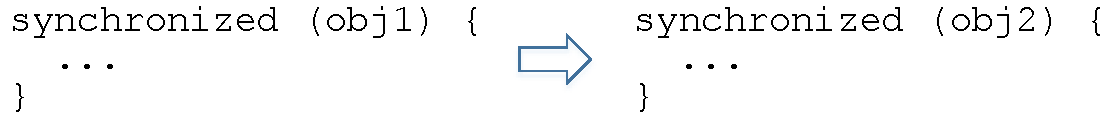
\includegraphics[scale=0.35]{pattern2}&6\\\hline
%		Changing critical section&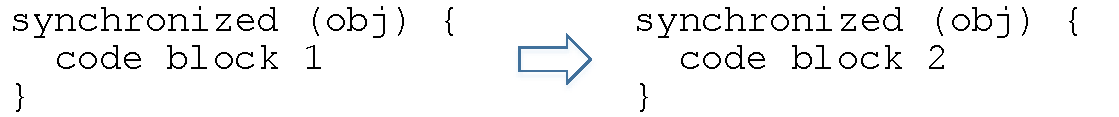
\includegraphics[scale=0.35]{pattern3}&35\\\hline
%		Adding or removing \texttt{volatile}&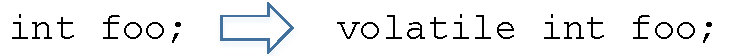
\includegraphics[scale=0.35]{pattern4}&47\\\hline
%		Thread-safe class replacement&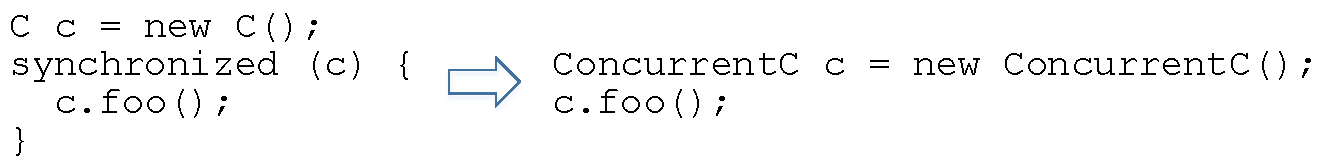
\includegraphics[scale=0.35]{pattern5}&32\\\hline
%		Thread management&&\\\hline
%		%Other class replacement&Some other concurrent related class replacement&\\\hline
%	\end{tabular}
%\end{table*}

%Switch to another type of lock
%Switch to another lock instace
%Change critical sections, which are protected by synchronization
%Add or remove 'volatile' modifier of a class field
%Use thread-safe class instead of handling concurrency control manually

%Table~\ref{} and \ref{} show an overview of our extracted change patterns. \zhong{Please explain the columns.}

Table~\ref{table:patterns} shows an overview of our extracted change patterns. Each row is an example of a certain change pattern. The first column is the sequence number of examples. The ``Source Code'' column shows the concrete source code of examples. The left is the original code and the right is the modified code. We align the corresponding statements. We use different colors to mark modified lines. The ``Simplified Code'' column shows the simplified code of the source code. They are short as they ignore the specific statements.

\begin{table*}
	\centering
\caption{Change patterns}\vspace*{-1ex}
	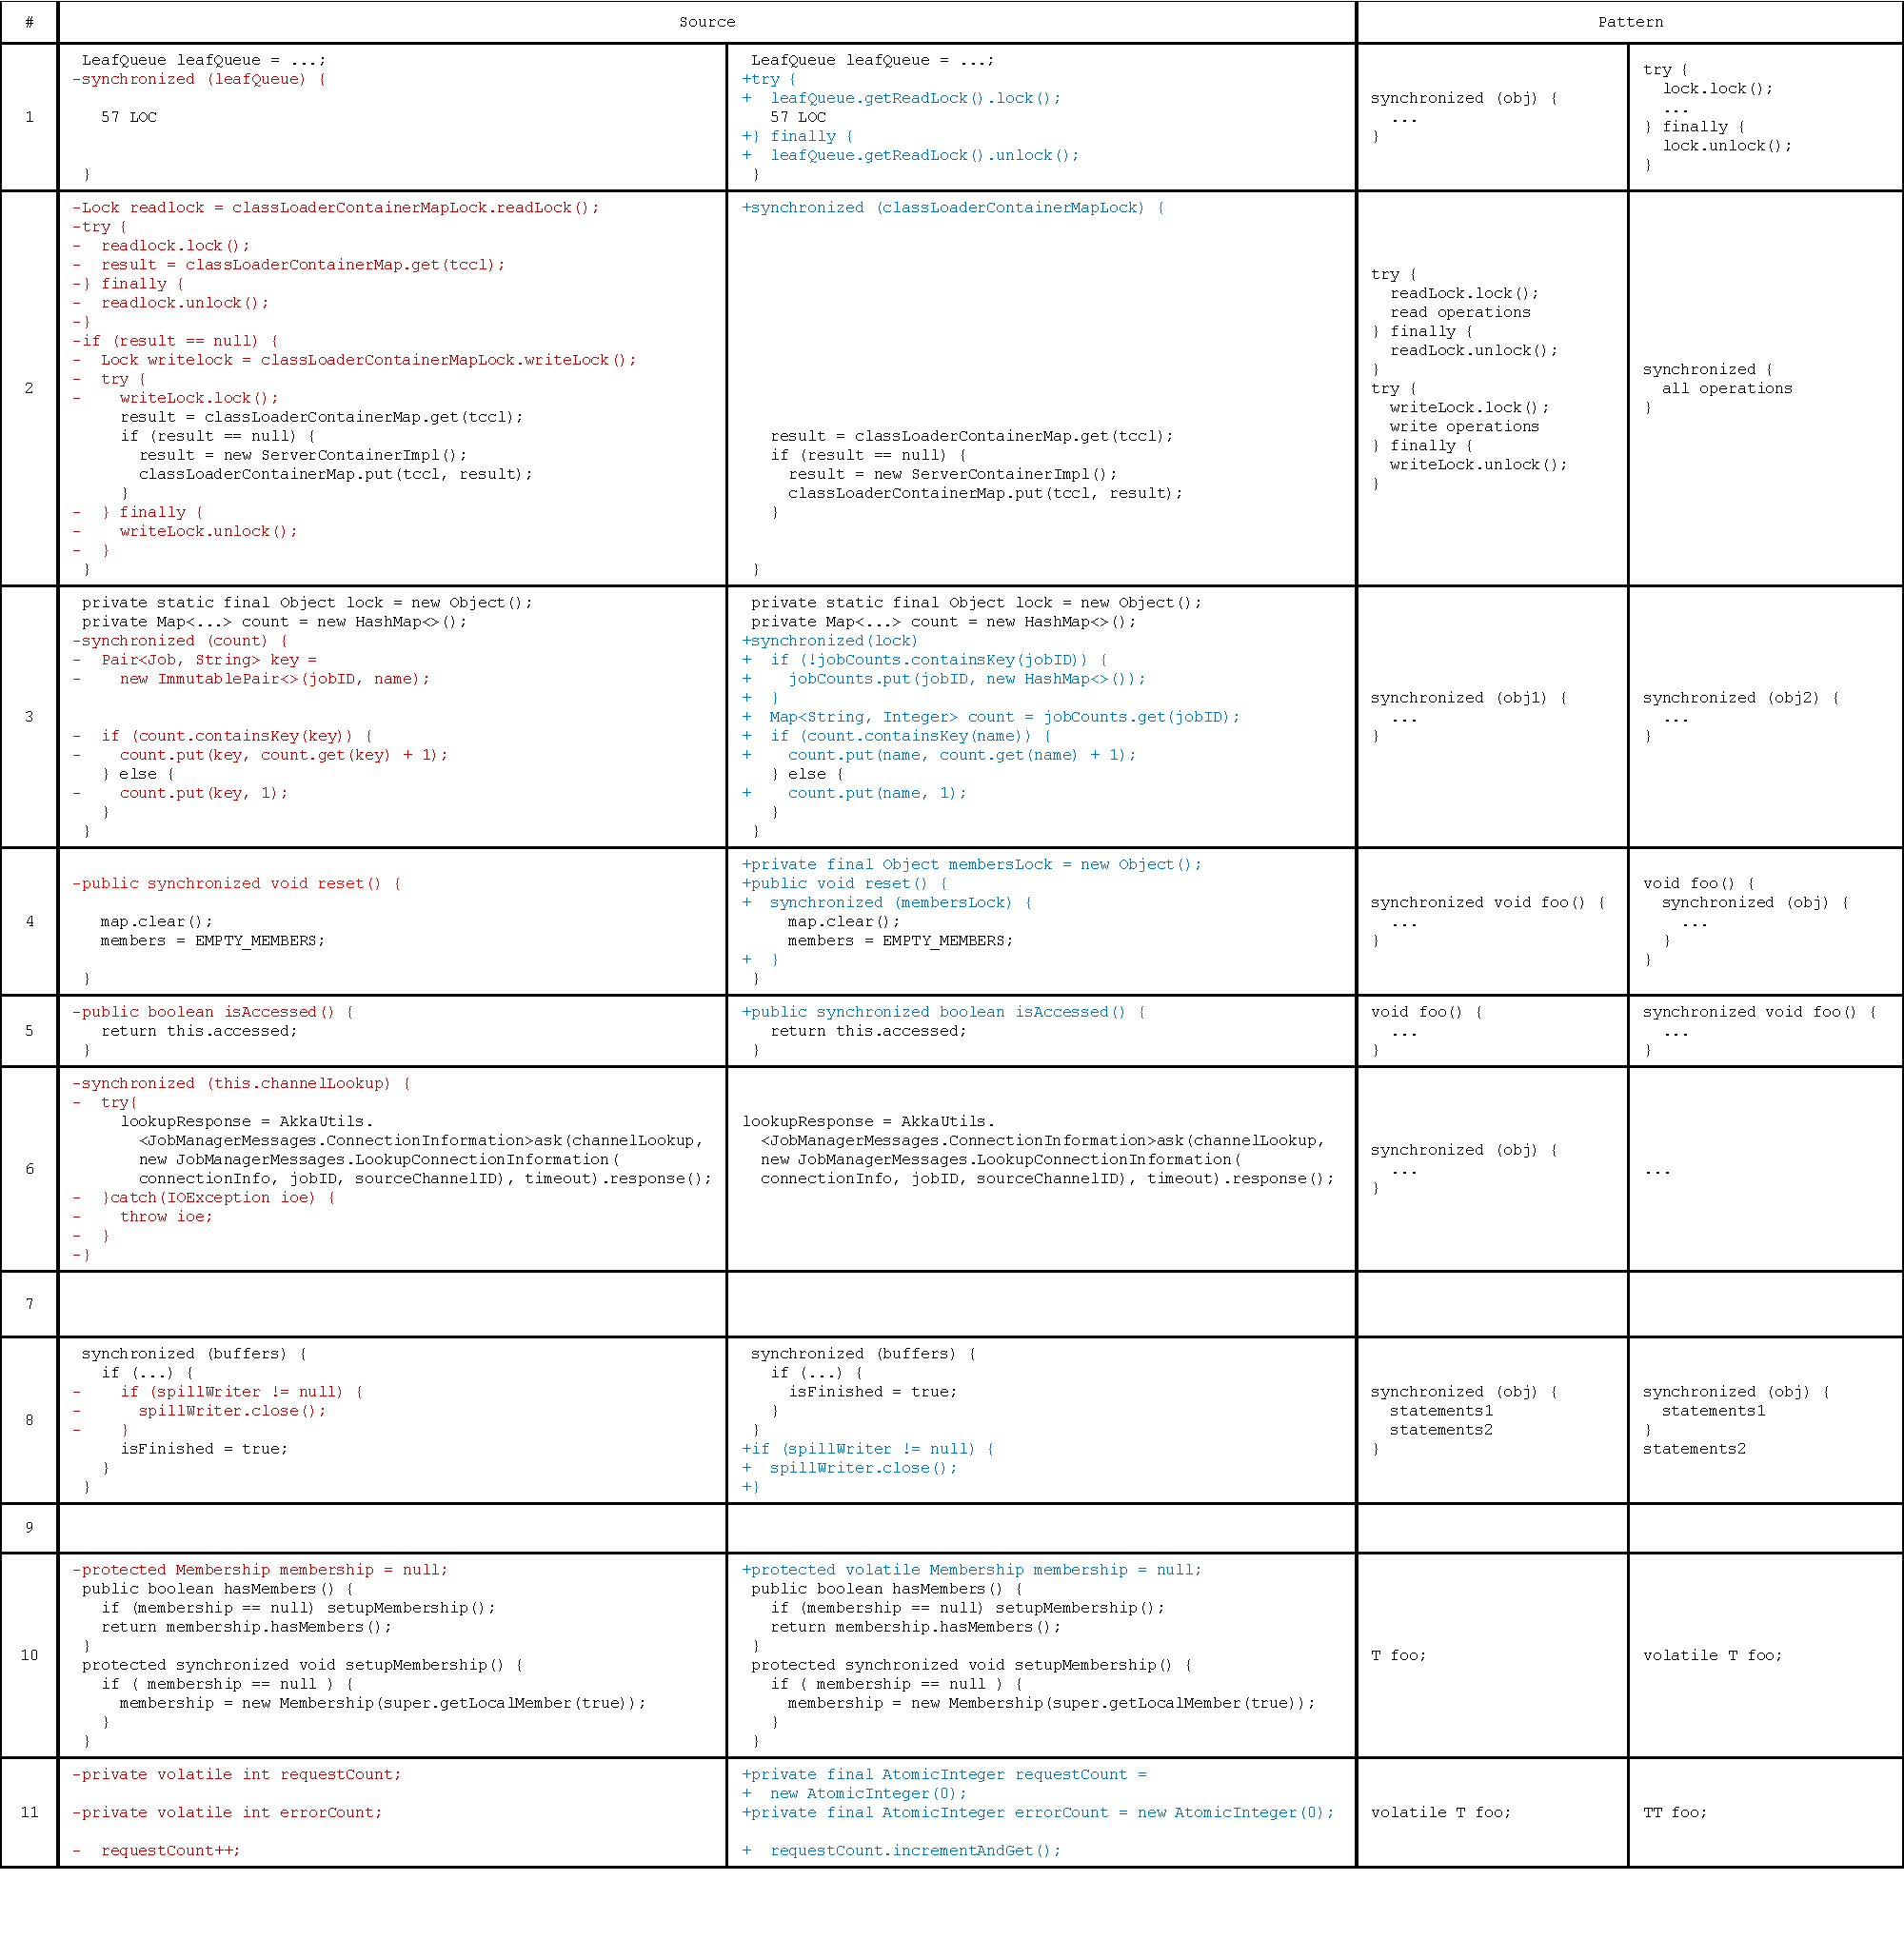
\includegraphics[width=1\textwidth]{patterns}	
	\label{table:patterns}\vspace*{-3ex}
\end{table*}

\noindent
\textbf{1. Changing lock types.} It is feasible to lock resources with different mechanisms. For example, Java has a keyword, \CodeIn{synchronized}. The keyword can lock a block of code lines. With the keyword, programmers do not have to acquire and release resources explicitly. Alternatively, programmers can explicitly lock resources with APIs (\emph{e.g.}, \CodeIn{ReentrantLock}). Explicit locks offer more features than the \CodeIn{synchronized} keyword does. For example, with such APIs, programmers can determine the conditions for a lock. As another example, besides exclusive locks, programmers can use shared locks. When a thread is holding an exclusive lock, other threads have to wait until it is released. In contrast, shared locks allow multiple threads to hold the lock with specific actions. For example, \CodeIn{ReadWriteLock} allows multiple read actions, but denies multiple write actions.%\zhong{Please explain what exclusive and shared locks are, and their benefits.}

%ReentrantLock, ReentrantReadWriteLock, StampedLock are all API level locks in Java. Although 'synchronized' keyword is convenient and straightforward, we need other locks when we have more requirements. ReentrantLock is a reentrant lock, which means a lock can be acquired repeatedly in the same thread. It is a exclusive lock with the similar behaviour as monitor lock but has more features such as fairness, condition and tryLock. ReadWriteLock is a pair of locks, which allows concurrent access to read operations when there is no write operation going on but exclusive access to write operations. StampedLock is a lock which provides three modes, namely writing, reading and optimistic reading. This lock is usually used in design of thread-safe classes.
%Programmers can change their lock types due to various considerations. For example, the \CodeIn{synchronized} keyword can fail to satisfy fairness (\zhong{What is fairness? Why does it matter?}), programmers have to change such implicit locks to explicit locks. \zhong{Add an example for each situation.}

We find that programmers can replace the \CodeIn{synchronized} keyword with parallel API classes. For example, the first item of Table~\ref{table:patterns} comes from YARN-5825\footnote{\url{https://issues.apache.org/jira/browse/YARN-5825} To save space, we remove the URLs of the other Apache issues. Their URLs can be built by replacing the above URL with their issue number.}. To improve the performance, programmers replaced the \CodeIn{synchronized} with the \CodeIn{getReadLock} method. The method returns a shared lock, so multiple threads can read the query simultaneously.

%3e4b1ae6dc786b268505aa2e64067432519c2bcf
%\begin{figure*}
%	\centering
%	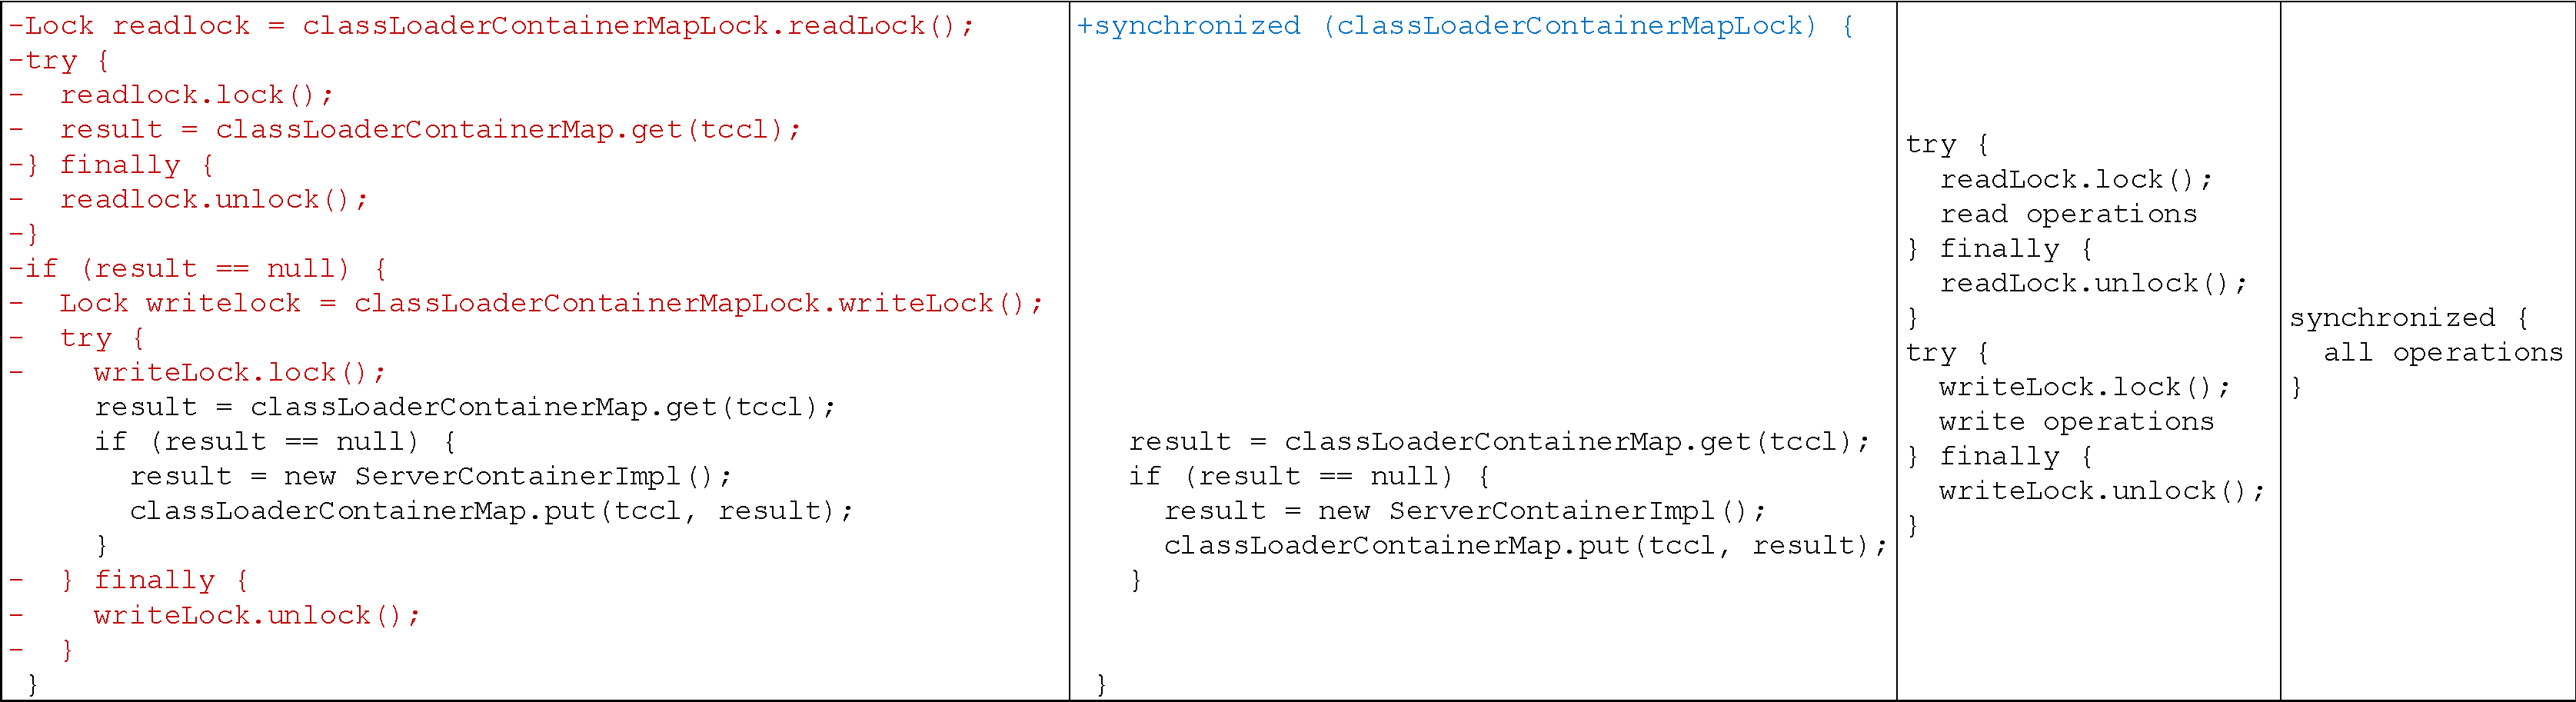
\includegraphics[scale=0.3]{locktype2}
%	\caption{Example 2}
%\zhong{It may be better, if you merge the example figures into a table like Table 1.}
%\end{figure*}

%\zhong{Please replace all texttt with CodeIn.}

%They also might switch to a reader-writer lock \cite{journals/cacm/CouroisHP71} from a normal lock to improve concurrency when there are plenty of concurrent read operations. Here are some examples. \zhong{add an example for this.}
Meanwhile, we find that programmers can replace parallel API classes with the \CodeIn{synchronized} keyword. For example, the second item of Table~\ref{table:patterns} comes from Tomcat\footnote{\url{https://svn.apache.org/viewvc?view=revision&revision=1414150}}. This commit is not reported, and we find it through our SVM classifier.% \zhong{List the commit message/log}.

%3e4b1ae6dc786b268505aa2e64067432519c2bcf
\begin{lstlisting}
A ReadWriteLock cannot be used to guard a WeakHashMap. The WeakHashMap may modify itself on get(), as it processes the reference queue of items removed by GC. Either a plain old lock / synchronization is needed, or some other solution.
\end{lstlisting}

As the above message explains, a developer complained that the \CodeIn{ReadWriteLock} method does not guard the \CodeIn{WeakHashMap} variable, since the \CodeIn{get()} method can modify the \CodeIn{WeakHashMap} variable, and the modification can bypass the lock. In this example, programmers fixed the problem by replacing the methods with the \CodeIn{synchronized} keyword.%todo more detail

%When they find that they only need a simple exclusive lock, they switch to synchronized block. \zhong{add an example for this}
%\begin{figure}
%	\centering
%	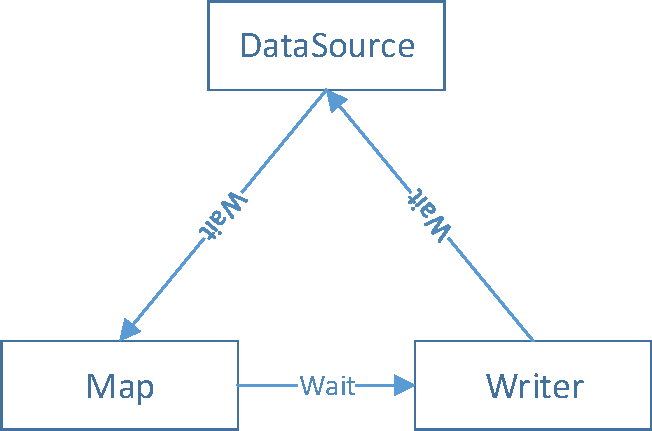
\includegraphics[height=1.7in]{deadlock}
%	\caption{Deadlock}
%	\label{figure:deadlock}
%%\zhong{Please add resource columns and add edges to denote resource manipulations.}
%\end{figure}

\noindent
\textbf{2. Changing locked variables.} A program needs to lock variables before it enters critical section bodies. During software maintenance, programmers can change locked variables, and we find that the main purpose is to repair bugs. For example, the third item of Table~\ref{table:patterns} comes from FLINK-1419. This bug complains that \CodeIn{DistributedCache} does not preserve files for subsequent operations. Based on its discussions, we understand that in the buggy file, programmers lock \CodeIn{count}, while they shall lock \CodeIn{lock}. To fully fix the bug, programmers also modified the critical sections and the \CodeIn{finally} clause.

As another example, when repairing bugs, programmers can add new locks. For example, the fourth item of Table~\ref{table:patterns} comes from Tomcat\footnote{\url{https://bz.apache.org/bugzilla/show\_bug.cgi?id=58386}}. It includes the following message:

\begin{lstlisting}
Reported by RV-Predict (a dynamic race detector) when running the test suite:
Data race on field org.apache.catalina.tribes.io.ObjectReader.accessed: {{{
Concurrent write in thread T93 (locks held: {...})
\end{lstlisting}

The data race indicates that the \CodeIn{isAccessed()} is not locked, so programmers add the \CodeIn{synchronized} keyword to allow locking on the method.


%We find that programmers can also delete unnecessary locks. For example, the fifth item of Table~\ref{table:patterns} comes from Flink:
%
%\begin{lstlisting}
%...Remove synchronized blcok in getReceiverList of ChannelManager which effectively serialized the connection lookup calls of a single task manager.
%\end{lstlisting}
%%\zhong{show the URL of the commit}.
%%\zhong{show what programmers say. Why it is unnecessary}.
%
%As the above commit messages says, programmers removed synchronization from the \CodeIn{ChannelManager} class to improve the performance.


%\zhong{show the URL of the commit}.
%\zhong{show what programmers say. Why it is unnecessary}.




%\zhong{Why do you present the above stack trace.}

%\zhong{Instead of why a deadlock occurs, you shall explain why the modification in Table~\ref{table:patterns2} repaired the deadlock. If the modification alone is insufficient, add more details here.}
%As shown in Figure~\ref{figure:deadlock}, a deadlock can occur when three threads execute in a specific order. Here, we use $s1$ and $s2$ to denote two statements. An arrow from $s1$ to $s2$ means $s1$ cannot be returned before $s2$ has been returned. The \CodeIn{DataSource} (thread-1) is waiting to be notified by the \CodeIn{Writer} (thread-2) when holding lock A. The \CodeIn{Writer} (thread-2) is trying to acquire lock B. But lock B is held by the \CodeIn{Map} (thread-3). And the \CodeIn{Map} (thread-3) is trying to acquire lock A, which is held by the \CodeIn{DataSource} (thread-1). Here is a waiting chain. This is a kind of bug known as deadlock. The problem is that the \CodeIn{DataSource} (thread-1) does not need to hold lock A while waiting to be notified. So the developer removed the unnecessary synchronization.

%f0e627bb8c9daedb3b064027cac37ce4849bab64
In some other cases, we find that programmers can refine their locked resources to improve performance. For example, the sixth item of Table~\ref{table:patterns} comes from Tomcat\footnote{\url{https://bz.apache.org/bugzilla/show_bug.cgi?id=58382}}. The original code locks the instance of a class, but the modified code locks only the \CodeIn{membersLock} field.

\noindent
\textbf{3. Modifications inside critical section bodies.} A critical section is a code block that is executed, when a thread locks the corresponding resources. We notice that even modifications inside critical section bodies can repair concurrency bugs. For example, the fifth item of Table~\ref{table:patterns} comes from FLINK-2384. It is caused by an implicit lock in the \CodeIn{spillWriter.close()} method. As programmers typically do not know such locks inside APIs, the lock leads to the deadlock. Indeed, we find that a recent benchmark~\cite{lin2015ase} includes a similar concurrency bug, and Lin \emph{et al.}~\cite{lin2016lockpeeker} proposed an approach that detects such implicit locks inside APIs. In this example, programmers move the \CodeIn{spillWriter.close()} method outside the critical section body to resolve the deadlock.

%
%\begin{lstlisting}
%"CHAIN DataSource (at createInput(ExecutionEnvironment.java:502) (org.apache.flink.api.java.hadoop.mapreduce.HadoopInputFormat)) -> FlatMap (FlatMap at readFlinkTuplesFromThriftParquet(ParquetThriftEntitons.java:96)) (7/8)" daemon prio=10 tid=0x00007f934005b000 nid=0x73c4 in Object.wait() [0x00007f93c16ac000]
%java.lang.Thread.State: TIMED_WAITING (on object monitor)
%
%"IOManager writer thread #1" daemon prio=10 tid=0x00007f93d8b7b000 nid=0x73a8 waiting for monitor entry [0x00007f93c2fc5000]
%java.lang.Thread.State: BLOCKED (on object monitor)
%
%"Map (Projection [0, 1, 2, 3, 4]) (7/8)" daemon prio=10 tid=0x00007f92b0434800 nid=0x74a3 waiting for monitor entry [0x00007f93a32f1000]
%java.lang.Thread.State: BLOCKED (on object monitor)
%\end{lstlisting}

%<<<<<<< HEAD
%f0e627bb8c9daedb3b064027cac37ce4849bab64
%In some other cases, we find that programmers can refine their locked resources to improve performance. For example, the seventh item of Table~\ref{table:patterns} comes from Tomcat\footnote{\url{https://bz.apache.org/bugzilla/show_bug.cgi?id=58382}}. The original code locks the instance of a class, but the modified code locks only the \CodeIn{membersLock} field.

%\noindent
%\textbf{3. Modifications on critical section bodies.} A critical section is a code block that is executed, when a thread locked the corresponding resources. The modifications on critical section bodies indicate new functionalities or refactoring. For example, the eighth item of Table~\ref{table:patterns2} comes from HDFS-4200. To reduce the size of a critical section body, programmers refactor the body into several methods. Indeed, this issue involves modifications that are related to even more change patterns (\emph{e.g.}, adding locked variables).
%=======
Besides the above example, the majority of modifications on critical section bodies indicates new functionalities or refactoring. For example, the seventh item of Table~\ref{table:patterns} comes from HDFS-4200. To reduce the size of a critical section body, programmers refactor the body into several methods. Indeed, this issue involves modifications that are related to even more change patterns (\emph{e.g.}, adding locked variables).
%>>>>>>> 9e8b767a2cf136027178c18c50d9c5eea616e630

%c93d9eaf363a535dff25cc4e7db400d879e73bb1
%Add option to use single actor system for local execution. Use local connection manager if a single task manager is used for local execution. Remove synchronized blcok in getReceiverList of ChannelManager which effectively serialized the connection lookup calls of a single task manager.
%\zhong{Why do you list the following commits? If you cannot list the following commit in Table~\ref{table:patterns2}, split it into the original code and fixed code. Explain them separatively.}

%Modifications on statements change statements of critical sections.

%efca79cfb7b496b4bec70561cc94af069c644ef2
%[FLINK-2384] [runtime] Move blocking I/O call outside of synchronized block
%Problem: Waiting on asynchronous write requests with the partition lock can
%result in a deadlock, because all other operations on the same partition are
%blocked. It is possible that the I/O writer itself needs to access the
%partition, in which cases the whole program blocks.
%Solution: Move the wait outside the synchronized block. This was not necessary
%before, because no operation assumes the spilling to be finished when the
%finish call has returned.




%Modifications on locked resources change the criteria of entering critical sections.  \zhong{Please check whether the samples explain the corresponding situations.}



%Example 9.



\noindent
\textbf{4. Changing the \CodeIn{volatile} keyword.} In Java, the \CodeIn{volatile} keyword denotes a variable that is saved in the main memory. For a \CodeIn{volatile} variable, a thread reads its latest value from the main memory, instead of the obsolete  value in the cache. Although it can improve the overall performance, races can occur, when multiple threads read and write \CodeIn{volatile} variables simultaneously.

%8313fa0f1ca277e9633a78f461804abc3c5515b8
%Fix https://bz.apache.org/bugzilla/show_bug.cgi?id=58392
%Double-checked locking needs to use volatile to be thread-safe
We find that programmers can add the \CodeIn{volatile} keyword to improve performance. For example, the eighth item of Table~\ref{table:patterns} comes from Tomcat\footnote{\url{https://bz.apache.org/bugzilla/show_bug.cgi?id=58392}}. It reports a data race, and the bug was repaired by adding the \CodeIn{volatile} keyword.

%560cd00890b3f6af2aca0c3a9d51a45f880692dd
%Fix a FindBugs warning (increment of volatile not atomic)

%\zhong{Please explain why you need two samples for this situation.}
Besides adding the keyword, we find that programmers have to remove the \CodeIn{volatile} keyword, since they do not fully understand its meanings. For example, in ninth item of Table~\ref{table:patterns} comes from Tomcat\footnote{\url{https://svn.apache.org/viewvc?view=revision&revision=1360946}}. In this bug, programmers auto-increment a \CodeIn{volatile} variable, but such an action is not atomic. As a result, FindBugs reports it as a bug, and programmers have to remove the keyword.

\noindent
\textbf{5. Replacing self-written code with Parallel APIs.} Programmers can implement concurrent code by themselves, but later they realize that it is easier to call APIs that already implement their functionalities. For example, a previous version of Hadoop has the following code:% \zhong{Replace the below commit with the buggy code.}


\begin{lstlisting}
private volatile long genstamp;
public synchronized long nextStamp() {
  this.genstamp++;
  return this.genstamp; }
\end{lstlisting}

Later, a programmer realized that it is better to replace the above code with the \CodeIn{AtomicLong} class. He reported the issue (HDFS-4029), and set its priority as major. Here, \CodeIn{AtomicLong} is a thread-safe version of type long. It allows updating a \CodeIn{Long} value without explicit synchronization and it is fast.

%It not only offers a simple interface, but also has a different implementation than the example code above. It uses \CodeIn{Unsafe} class, which provides unsafe operations as its name represents. This class allows low-level programming in Java, which is considered unsafe but can save running time without the check to guarantee safety. It might be promoted to be public API in Java 9. The fixed code is as follow:

%\zhong{Replace the below commit with the fixed code.}

\begin{lstlisting}
private volatile long genstamp;
public long nextStamp() {
  return genstamp.incrementAndGet(); }
\end{lstlisting}

Besides replacing directly, programmers can replace their code with parallel APIs that implement similar functions. For example, the below code comes from LUCENE-2779:

\begin{lstlisting}
protected ... fileMap = new HashMap<...>();
public final boolean fileExists(String name) {
  ensureOpen();
  RAMFile file;
  synchronized (this) { file = fileMap.get(name); }
  return file != null; }
\end{lstlisting}

Instead of handling synchronization by themselves, programmers replaced the above code with a parallel API:

\begin{lstlisting}
protected ... fileMap = new ConcurrentHashMap<...>();
public final boolean fileExists(String name) {
  ensureOpen();
  return fileMap.containsKey(name); }
\end{lstlisting}

%\textbf{Other class replace}
%
%\textbf{Thread resource management}
%
%When we do concurrent programming, we need to pay attention to resource management such as threads, locks.
%
%Thread management is to deal with the management of thread-related resources.
%
%\textbf{Thread sleep wait notify}
%
%It is a another way of synchronization which is less common than locking.
%
%\textbf{Final in multiple threads}

In summary, we identify five types of change patterns in total. The percentages of their occurrence are 4\%, 3.5\%, 29\%, 34.5\% and 29\% respectively. First, we find that programmers can modify parallel keywords and locked variables, and such modifications are mainly for repairing bugs and improving performance. Second, we notice modifications on critical section bodies, and such modifications often indicate new functions. Finally, we notice that self-written code is replaced with corresponding parallel APIs. In most cases, we find that maintaining concurrent code is not a one-direction migration. For example, there are several different ways to implement a lock. Programmers shall carefully analyze their programming contexts to determine which is their best choice. As shown in our examples, during software maintenance, programmers can migrate to any types according to their need.

\subsection{RQ2. The usefulness of our change patterns.}
\label{sec:result:sample}

%\zhong{Try to add an example for each change pattern.}
%\zhong{How many pull requests did you submit?}

Once developers know and understand these change patterns well in concurrent programming, they can refer to these change patterns to see whether one of them matches the condition when they are writing or maintaining concurrent code and then make the change. However, it is impractical for us to read vast concurrent code and find examples to apply the change patterns. Instead, we use a keyword search method to find possible code context to apply the change patterns.

In total, we made three pull requests. We made the first pull request on Schmince-2\footnote{\url{https://github.com/derekmu/Schmince-2}}. This is a game, where players control space tourists for adventure. It has the following code:

\begin{lstlisting}
public class DRandom {
  private ... random = new ThreadLocal<Random>() {
    protected Random initialValue() {return new Random();}};
  public static Random get() {return random.get();}}
\end{lstlisting}

The above code implements a class that generates random values for multiple threads. We find that J2SE provides the \CodeIn{ThreadLocalRandom} class\footnote{\url{https://docs.oracle.com/javase/8/docs/api/java/util/concurrent/ThreadLocalRandom.html}} that implements the identical function. According to our fifth change pattern, we made a pull request to replace the above code with the corresponding API\footnote{\url{https://github.com/derekmu/Schmince-2/pull/1}}. This pull request is already confirmed.
%\begin{lstlisting}
%+import java.util.concurrent.ThreadLocalRandom;
%public class DRandom {
%-    private static ThreadLocal<Random> random = new ThreadLocal<Random>() {
%-        protected Random initialValue() {
%-            return new Random();
%-        }
%-    };
%public static Random get() {
%-        return random.get();
%+        ThreadLocalRandom.current();
%}
%}
%\end{lstlisting}

%This example shows a change from ThreadLocal$<$Random$>$ to ThreadLocalRandom from JDK7. It is from a Schmince-2, a game on Google Play. We make the change and our pull request\footnote{\url{https://github.com/derekmu/Schmince-2/pull/1}} has been accept. ThreadLocalRandom should be used when available in place of ThreadLocal$<$Random$>$. For JDK7 the difference is minimal, but JDK8 starts including optimizations for ThreadLocalRandom. The ThreadLocal class provides thread-local variables. The ThreadLocalRandom class is a random number generator isolated to the current thread.

We made the second pull request on UnifiedEmail\footnote{\url{https://github.com/HexagonRom/android_packages_apps_UnifiedEmail}}. It is an Android email client. It has the following code:

\begin{lstlisting}
static NMap map = null;
static synchronized NMap getNMap(Context context) {
  if (map == null) {
    map = new NMap();
    map.loadNotificationMap(context); }
  return map; }
\end{lstlisting}

If the \CodeIn{map} field is \CodeIn{null}, the above method creates a new map and assigns the new map to the field. To allow multiple threads to call the methods, programmers add the \CodeIn{synchronized} keyword to the method. We believe that when \CodeIn{map} is not \CodeIn{null}, the lock is unnecessary, since it does not change the field. According to our second change pattern, we made the following modification to synchronize only the lines that modify the field:

\begin{lstlisting}
static volatile NMap map = null;
static NMap getNMap(Context context) {
  if (map == null) {
    synchronized (NotificationUtils.class) {
      if (map == null) {
        map = new NMap();
        map.loadNotificationMap(context); }}}
  return map; }
\end{lstlisting}

%The above pull request is still pending.
The owner of the project deleted our pull request. We checked the pull requests of the project and found that there is no open or closed pull request. This project has more than 19,000 commits. It is possible that it has a strict policy of introducing external source code.



We made the third pull request on Spider4java\footnote{\url{https://github.com/lichangshu/spider4java}}. It is a Java web crawler. It has the following code:

\begin{lstlisting}
public class Counter {
  protected int count;
  public Counter() { count = 0; }
  public synchronized void increment() {count=count+1;}
  public synchronized int getValue() {return count;}}
\end{lstlisting}

The above class implements a counter for multiple threads. As J2SE provides the identical API, \CodeIn{AtomicInteger}\footnote{\url{https://docs.oracle.com/javase/8/docs/api/java/util/concurrent/atomic/AtomicInteger.html}}. Our pull request has been accepted, and its code is as follow:

\begin{lstlisting}
public class Counter {
  protected AtomicInteger count;
  public Counter() { count = new AtomicInteger(); }
  public void increment() { count.getAndIncrement(); }
  public int getValue() { return count.get(); }}
\end{lstlisting}




%However, their programmers denied the pull request. Although our pull request works, it is more neat to systematically replace the above \CodeIn{Counter} class with the \CodeIn{AtomicInteger} class. Their programmers may deny our pull request, simply because the wrapper style looks ugly.

In summary, our results show that our change patterns are repetitive in future maintenance, and programmers confirmed that our change patterns are useful. However, our results also reveal that it needs much programming experience to fully unleash the potential of our change patterns. We further discuss this issue in Section~\ref{sec:discuss}.



\subsection{Threats to Validity}

The threats to internal validity include that our tool can omit some concurrency commits. Although we have used both the query-based search and a classifier in our study, our tool may fail to identify all concurrency commits. We did not conduct a thorough evaluation on our classifier. The threat could be reduced by more advanced identification techniques. The threats to internal validity also include obsolete commits. With the rapid development of software, such commits may present obsolete or even wrong usages. To reduce the threat, in our study, we prefer to recent commits. The threats to external validity include our selected projects and programming language. The number of the projects we select is small. They are all Java-based Apache projects. The threat could be reduced by introducing more projects and languages in future work.

